% answers.tex —— 2006 年·普通高等学校招生考试·湖北卷理科 · 参考答案与详细解析片段
% 由 tools/generate_projects.py 依来源总账自 2006/2006_数学真题_湖北理_试题.md + 2006/2006_数学真题_湖北理_解析正文.md + 2006/2006_数学真题_湖北理_答案要点.md 生成，勿手改（改源 MD 后重跑）


\begin{gktip}
以下为依据固定候选题面独立求解的草稿，不是官方答案或解析。未使用未核验的答案材料。题面来源身份未核；Q17（2）照录题面并保留无解结论，不猜测原题意图。
\end{gktip}

\begin{answer}
\gksolhead{1}{}

\textbf{题目}：

已知向量 $\vec a=(\sqrt3,1)$，$\vec b$ 是不平行于 $x$ 轴的单位向量，且 $\vec a\cdot\vec b=\sqrt3$，则 $\vec b=$\mbox{（　　）}

\begin{gkopts}(2)
\task （A）$\left(\dfrac{\sqrt3}{2},\dfrac12\right)$
\task （B）$\left(\dfrac12,\dfrac{\sqrt3}{2}\right)$
\task （C）$\left(\dfrac14,\dfrac{3\sqrt3}{4}\right)$
\task （D）$(1,0)$
\end{gkopts}

\Needspace{4\baselineskip}
\textbf{解析}

设 $\vec b=(u,v)$。由 $\sqrt3u+v=\sqrt3$、$u^2+v^2=1$，得 $\vec b=(1,0)$ 或 $(1/2,\sqrt3/2)$。题设排除平行 $x$ 轴者，选 B。

\gkanswer{答案：B。}

\end{answer}
\begin{answer}
\gksolhead{2}{}

\textbf{题目}：

若互不相等的实数 $a,b,c$ 成等差数列，$c,a,b$ 成等比数列，且 $a+3b+c=10$，则 $a=$\mbox{（　　）}

\begin{gkopts}(4)
\task （A）$4$
\task （B）$2$
\task （C）$-2$
\task （D）$-4$
\end{gkopts}

\Needspace{4\baselineskip}
\textbf{解析}

等差条件给 $a+c=2b$，结合 $a+3b+c=10$ 得 $b=2,a+c=4$。等比条件 $a^2=bc=2c$ 与 $a+c=4$ 给 $a=2$ 或 $-4$；$a=2$ 使三数相等，不符合互不相等，故 $a=-4$，选 D。

\gkanswer{答案：D（$a=-4$）。}

\end{answer}
\begin{answer}
\gksolhead{3}{}

\textbf{题目}：

$\triangle ABC$ 的内角 $A$ 满足 $\sin 2A=\dfrac23$，则 $\sin A+\cos A=$\mbox{（　　）}

\begin{gkopts}(2)
\task （A）$\dfrac{\sqrt{15}}3$
\task （B）$-\dfrac{\sqrt{15}}3$
\task （C）$\dfrac53$
\task （D）$-\dfrac53$
\end{gkopts}

\Needspace{4\baselineskip}
\textbf{解析}

$A\in(0,\pi)$ 且 $\sin2A>0$，故 $A\in(0,\pi/2)$。于是 $(\sin A+\cos A)^2=1+\sin2A=5/3$，取正根，选 A。

\gkanswer{答案：A（$\sqrt{15}/3$）。}

\end{answer}
\begin{answer}
\gksolhead{4}{}

\textbf{题目}：

设 $f(x)=\lg\dfrac{2+x}{2-x}$，则 $f\left(\dfrac{x}{2}\right)+f\left(\dfrac{2}{x}\right)$ 的定义域为\mbox{（　　）}

（A）$(-4,0)\cup(0,4)$　（B）$(-4,-1)\cup(1,4)$

（C）$(-2,-1)\cup(1,2)$　（D）$(-4,-2)\cup(2,4)$

\Needspace{4\baselineskip}
\textbf{解析}

两个对数的真数条件合并为 $|x/2|<2$、$|2/x|<2$，即 $1<|x|<4$，选 B。

\gkanswer{答案：B。}

\end{answer}
\begin{answer}
\gksolhead{5}{}

\textbf{题目}：

在 $\left(\sqrt{x}-\dfrac{1}{\sqrt[3]{x}}\right)^{24}$ 的展开式中，$x$ 的幂的指数是整数的项共有\mbox{（　　）}

\begin{gkopts}(4)
\task （A）$3$ 项
\task （B）$4$ 项
\task （C）$5$ 项
\task （D）$9$ 项
\end{gkopts}

\Needspace{4\baselineskip}
\textbf{解析}

展开通项中 $x$ 的指数为 $12-5k/6$，其中 $k=0,1,\ldots,24$。指数为整数当且仅当 $k$ 是 $6$ 的倍数，共 $5$ 项，选 C。

\gkanswer{答案：C（5 项）。}

\end{answer}
\begin{answer}
\gksolhead{6}{}

\textbf{题目}：

关于直线 $m,n$ 与平面 $\alpha,\beta$，有以下四个命题：

① 若 $m\parallel\alpha$，$n\parallel\beta$ 且 $\alpha\parallel\beta$，则 $m\parallel n$；

② 若 $m\perp\alpha$，$n\perp\beta$ 且 $\alpha\perp\beta$，则 $m\perp n$；

③ 若 $m\perp\alpha$，$n\parallel\beta$ 且 $\alpha\parallel\beta$，则 $m\perp n$；

④ 若 $m\parallel\alpha$，$n\perp\beta$ 且 $\alpha\perp\beta$，则 $m\parallel n$。

其中真命题的序号是\mbox{（　　）}

\begin{gkopts}(4)
\task （A）①②
\task （B）③④
\task （C）①④
\task （D）②③
\end{gkopts}

\Needspace{4\baselineskip}
\textbf{解析}

①两平面平行时，分别平行于两平面的直线方向未必相同，假；②两直线分别沿两互相垂直平面的法向，故互相垂直，真；③$\alpha\parallel\beta$ 且 $n\parallel\beta$ 给出 $n$ 的方向平行于 $\alpha$，而 $m\perp\alpha$，故垂直，真；④$\alpha\perp\beta$ 只使 $n$ 的方向落在 $\alpha$ 内，$m$ 也可取该平面内不同方向，假。选 D（②③）。

\gkanswer{答案：D（②③）。}

\end{answer}
\begin{answer}
\gksolhead{7}{}

\textbf{题目}：

设过点 $P(x,y)$ 的直线分别与 $x$ 轴的正半轴和 $y$ 轴的正半轴交于 $A,B$ 两点，点 $Q$ 与点 $P$ 关于 $y$ 轴对称，$O$ 为坐标原点，若 $\overrightarrow{BP}=2\overrightarrow{PA}$ 且 $\overrightarrow{OQ}\cdot\overrightarrow{AB}=1$，则点 $P$ 的轨迹方程是\mbox{（　　）}

（A）$3x^2+\dfrac32y^2=1\ (x>0,y>0)$　（B）$3x^2-\dfrac32y^2=1\ (x>0,y>0)$

（C）$\dfrac32x^2-3y^2=1\ (x>0,y>0)$　（D）$\dfrac32x^2+3y^2=1\ (x>0,y>0)$

\Needspace{4\baselineskip}
\textbf{解析}

设 $A=(u,0),B=(0,v),P=(x,y)$。由 $\overrightarrow{BP}=2\overrightarrow{PA}$ 得 $3P=2A+B$，即 $u=3x/2,v=3y$。又 $Q=(-x,y)$，于是 $\overrightarrow{OQ}\cdot\overrightarrow{AB}=xu+yv=1$，得到 $3x^2/2+3y^2=1$，选 D。

\gkanswer{答案：D。}

\end{answer}
\begin{answer}
\gksolhead{8}{}

\textbf{题目}：

有限集合 $S$ 中元素的个数记作 $\operatorname{card}(S)$，设 $A,B$ 都为有限集合，给出下列命题：

① $A\cap B=\varnothing$ 的充要条件是 $\operatorname{card}(A\cup B)=\operatorname{card}(A)+\operatorname{card}(B)$；

② $A\subseteq B$ 的必要条件是 $\operatorname{card}(A)\leqslant\operatorname{card}(B)$；

③ $A\nsubseteq B$ 的充分条件是 $\operatorname{card}(A)\leqslant\operatorname{card}(B)$；

④ $A=B$ 的充要条件是 $\operatorname{card}(A)=\operatorname{card}(B)$。

其中真命题的序号是\mbox{（　　）}

\begin{gkopts}(4)
\task （A）①③④
\task （B）①②
\task （C）①④
\task （D）②③
\end{gkopts}

\Needspace{4\baselineskip}
\textbf{解析}

有限集有 $|A\cup B|=|A|+|B|-|A\cap B|$，故①真；$A\subseteq B$ 必有 $|A|\le|B|$，故②真。③、④可由不同但同基数的有限集反驳。选 B（①②）。

\gkanswer{答案：B（①②）。}

\end{answer}
\begin{answer}
\gksolhead{9}{}

\textbf{题目}：

已知平面区域 $D$ 由以 $A(1,3),B(5,2),C(3,1)$ 为顶点的三角形内部和边界组成。若在区域 $D$ 上有无穷多个点 $(x,y)$ 可使目标函数 $z=x+my$ 取得最小值，则 $m=$\mbox{（　　）}

\begin{gkopts}(4)
\task （A）$-2$
\task （B）$-1$
\task （C）$1$
\task （D）$4$
\end{gkopts}

\Needspace{4\baselineskip}
\textbf{解析}

目标向量 $(1,m)$ 要与边 $AC$ 平行，才会在整条边上取相同值。$C-A=(2,-2)$，故 $1-m=0$，即 $m=1$。此时 $z(A)=z(C)=4<z(B)=7$，确为最小边，选 C。

\gkanswer{答案：C（$m=1$）。}

\end{answer}
\begin{answer}
\gksolhead{10}{}

\textbf{题目}：

关于 $x$ 的方程 $(x^2-1)^2-|x^2-1|+k=0$，给出下列四个命题：

① 存在实数 $k$，使得方程恰有 $2$ 个不同的实根；

② 存在实数 $k$，使得方程恰有 $4$ 个不同的实根；

③ 存在实数 $k$，使得方程恰有 $5$ 个不同的实根；

④ 存在实数 $k$，使得方程恰有 $8$ 个不同的实根。

其中假命题的个数是\mbox{（　　）}

\begin{gkopts}(4)
\task （A）$0$
\task （B）$1$
\task （C）$2$
\task （D）$3$
\end{gkopts}

\Needspace{4\baselineskip}
\textbf{解析}

令 $u=|x^2-1|\ge0$，方程化为 $u^2-u+k=0$。取 $k$ 分别为 $-1,1/4,0$ 及 $0<k<1/4$，可分别得到 $2,4,5,8$ 个不同实根。因此四个命题都真，假命题数为 $0$，选 A。

\gkanswer{答案：A（假命题数为 0）。}

\end{answer}
\begin{answer}
\gksolhead{11}{}

\textbf{题目}：

\Needspace{5\baselineskip}
设 $x,y$ 为实数，且
\nopagebreak[4]
\[
\frac{x}{1-i}+\frac{y}{1-2i}=\frac{5}{1-3i},
\]
则 $x+y=$ \gkblank{}。

\Needspace{4\baselineskip}
\textbf{解析}

\Needspace{5\baselineskip}
分别有理化各分母并比较实、虚部：
\nopagebreak[4]
\[
\frac{x}{1-i}=\frac{x(1+i)}2,\quad
\frac{y}{1-2i}=\frac{y(1+2i)}5,\quad
\frac5{1-3i}=\frac{5(1+3i)}{10}.
\]

得到 $x/2+y/5=1/2$、$x/2+2y/5=3/2$，解得 $x=-1,y=5$，故 $x+y=4$。

\gkanswer{答案：$4$。}

\end{answer}
\begin{answer}
\gksolhead{12}{}

\textbf{题目}：

接种某疫苗后，出现发热反应的概率为 $0.80$，现有 $5$ 人接种该疫苗，至少有 $3$ 人出现发热反应的概率为 \gkblank{}。（精确到 $0.01$）

\Needspace{4\baselineskip}
\textbf{解析}

\Needspace{5\baselineskip}
令 $X$ 为发热人数，则 $X\sim B(5,0.8)$。所求概率为
\nopagebreak[4]
\[
\binom53(0.8)^3(0.2)^2+\binom54(0.8)^4(0.2)+(0.8)^5=0.94208\approx0.94.
\]

\gkanswer{答案：$0.94$。}

\end{answer}
\begin{answer}
\gksolhead{13}{}

\textbf{题目}：

已知直线 $5x+12y+a=0$ 与圆 $x^2-2x+y^2=0$ 相切，则 $a$ 的值为 \gkblank{}。

\Needspace{4\baselineskip}
\textbf{解析}

圆心为 $(1,0)$，半径为 $1$。圆心到直线距离条件为 $|5+a|/13=1$，解得 $a=8$ 或 $-18$。

\gkanswer{答案：$8$ 或 $-18$。}

\end{answer}
\begin{answer}
\gksolhead{14}{}

\textbf{题目}：

某工程队有 $6$ 项工程需要先后单独完成，其中工程乙必须在工程甲完成后才能进行，工程丙必须在工程乙完成后才能进行，又工程丁必须在工程丙完成后立即进行。那么安排这 $6$ 项工程的不同排法种数是 \gkblank{}。（用数字作答）

\Needspace{4\baselineskip}
\textbf{解析}

将“丙、丁”合为一个有序相邻块；甲、乙、该块三者内部先后顺序固定。连同另外两项共五个对象，排列数为 $5!/3!=20$。

\gkanswer{答案：$20$。}

\end{answer}
\begin{answer}
\gksolhead{15}{}

\textbf{题目}：

\Needspace{5\baselineskip}
将杨辉三角中的每一个数 $C_n^r$ 都换成分数 $\dfrac{1}{(n+1)C_n^r}$，就得到一个如下图所示的分数三角形，成为莱布尼茨三角形。从莱布尼茨三角形可看出
\nopagebreak[4]
\[
\frac{1}{(n+1)C_n^r}+\frac{1}{(n+1)C_n^{r+1}}=\frac{1}{nC_{n-1}^r},
\]
\Needspace{5\baselineskip}
其中 $x=\dfrac{1}{nC_{n-1}^r}$。令
\nopagebreak[4]
\[
a_n=\frac13+\frac1{12}+\cdots+\frac{1}{nC_{n-1}^{2}}+\frac{1}{(n+1)C_n^{2}},
\]
则 $\displaystyle\lim_{n\to\infty}a_n=$ \gkblank{}。
\nopagebreak[4]
\begin{center}% 2006 湖北理科第15题：源图中的莱布尼茨三角形分数排列。
\begin{tikzpicture}[x=0.86cm, y=0.78cm, font=\small]
  \node at (0, 0) {$\dfrac{1}{1}$};

  \node at (-0.5, -1) {$\dfrac{1}{2}$};
  \node at ( 0.5, -1) {$\dfrac{1}{2}$};

  \node at (-1, -2) {$\dfrac{1}{3}$};
  \node at ( 0, -2) {$\dfrac{1}{6}$};
  \node at ( 1, -2) {$\dfrac{1}{3}$};

  \node at (-1.5, -3) {$\dfrac{1}{4}$};
  \node at (-0.5, -3) {$\dfrac{1}{12}$};
  \node at ( 0.5, -3) {$\dfrac{1}{12}$};
  \node at ( 1.5, -3) {$\dfrac{1}{4}$};

  \node at (-2, -4) {$\dfrac{1}{5}$};
  \node at (-1, -4) {$\dfrac{1}{20}$};
  \node at ( 0, -4) {$\dfrac{1}{30}$};
  \node at ( 1, -4) {$\dfrac{1}{20}$};
  \node at ( 2, -4) {$\dfrac{1}{5}$};

  \node at (-2.5, -5) {$\dfrac{1}{6}$};
  \node at (-1.5, -5) {$\dfrac{1}{30}$};
  \node at (-0.5, -5) {$\dfrac{1}{60}$};
  \node at ( 0.5, -5) {$\dfrac{1}{60}$};
  \node at ( 1.5, -5) {$\dfrac{1}{30}$};
  \node at ( 2.5, -5) {$\dfrac{1}{6}$};

  \node at (-3, -6) {$\dfrac{1}{7}$};
  \node at (-2, -6) {$\dfrac{1}{42}$};
  \node at (-1, -6) {$\dfrac{1}{105}$};
  \node at ( 0, -6) {$\dfrac{1}{140}$};
  \node at ( 1, -6) {$\dfrac{1}{105}$};
  \node at ( 2, -6) {$\dfrac{1}{42}$};
  \node at ( 3, -6) {$\dfrac{1}{7}$};

  \node at (0, -7) {$\cdots\cdots$};
\end{tikzpicture}
\end{center}
\nopagebreak[4]
\Needspace{4\baselineskip}
\textbf{解析}

\Needspace{5\baselineskip}
恒等式右端的第 $k$ 项可写成
\nopagebreak[4]
\[
\frac1{k\binom{k-1}{2}}=\frac1{(k-1)(k-2)}-\frac1{k(k-1)}.
\]

故 $a_n$ 为望远镜和，极限为 $1/2$。

\gkanswer{答案：$1/2$。}

\end{answer}
\begin{answer}
\gksolhead{16}{}

\textbf{题目}：

\Needspace{5\baselineskip}
设函数
\nopagebreak[4]
\[
f(x)=\vec a\cdot(\vec b+\vec c),\quad
\vec a=(\sin x,-\cos x),\quad
\vec b=(\sin x,-3\cos x),\quad
\vec c=(-\cos x,\sin x),\quad x\in\mathbb R.
\]

（1） 求函数 $f(x)$ 的最大值和最小正周期；

（2） 将函数 $f(x)$ 的图像按向量 $\vec d$ 平移，使平移后得到的图像关于坐标原点成中心对称，求长度最小的 $\vec d$。

\Needspace{4\baselineskip}
\textbf{解析}

\gksubpart{(1)}

向量点积化简为 $f(x)=2+\cos2x-\sin2x$。振幅为 $\sqrt2$，最大值 $2+\sqrt2$，最小正周期 $\pi$。

\gksubpart{(2)}

将图像按 $(h,k)$ 平移后得到 $g(x)=f(x-h)+k$。常数项要求 $k=-2$。振荡部分关于原点为奇函数要求余弦项系数为零，即 $\cos2h+\sin2h=0$，所以 $h=-\pi/8+n\pi/2$。取绝对值最小的水平分量 $h=-\pi/8$，得到唯一的最短向量 $(-\pi/8,-2)$。

\gkanswer{答案（1）：最大值 $2+\sqrt2$，最小正周期 $\pi$。}

\gkanswer{答案（2）：最短平移向量为 $(-\pi/8,-2)$。}

\end{answer}
\begin{answer}
\gksolhead{17}{}

\textbf{题目}：

已知二次函数 $y=f(x)$ 的图象经过坐标原点，其导函数为 $f'(x)=6x-2$，数列 $\{a_n\}$ 的前 $n$ 项和为 $S_n$，点 $(n,S_n)\ (n\in\mathbb N^*)$ 均在函数 $y=f(x)$ 的图象上。

（1） 求数列 $\{a_n\}$ 的通项公式；

（2） 设 $b_n=\dfrac{m}{a_na_{n+1}}$，$T_n$ 是数列 $\{b_n\}$ 的前 $n$ 项和，求使得 $T_n<\dfrac{m}{20}$ 对所有 $n\in\mathbb N^*$ 都成立的最小正整数 $m$。

\Needspace{4\baselineskip}
\textbf{解析}

\gksubpart{(1)}

原函数 $f(x)=3x^2-2x$，故 $S_n=f(n)=3n^2-2n$，相邻差 $a_n=S_n-S_{n-1}=6n-5$。特别地 $a_1=1,a_2=7$。

\gksubpart{(2)}

$T_1=b_1=m/(a_1a_2)=m/7$。对任意正整数 $m$ 都有 $m/7>m/20$，已与题设要求的 $T_1<m/20$ 矛盾。因此按固定题面不存在这样的正整数 $m$，答案保留 U/PENDING，需外部可靠勘误或同版材料裁决。

\gkanswer{答案（1）：$a_n=6n-5$。}

\gkanswer{答案（2）：U/PENDING；}

\end{answer}
\begin{answer}
\gksolhead{18}{}

\textbf{题目}：

如图，在棱长为 $1$ 的正方体 $ABCD-A_1B_1C_1D_1$ 中，$P$ 是侧棱 $CC_1$ 上的一点，$CP=m$。

（1） 试确定 $m$，使直线 $AP$ 与平面 $BDD_1B_1$ 所成角的正切值为 $3\sqrt2$；

（2） 在线段 $A_1C_1$ 上是否存在一个定点 $Q$，使得对任意的 $m$，$D_1Q$ 在平面 $APD_1$ 上的射影垂直于 $AP$，并证明你的结论。
\nopagebreak[4]
\begin{center}% 2006 湖北理科第18题：源图所示正方体及上底面对角线；点 P 未画在源图中。
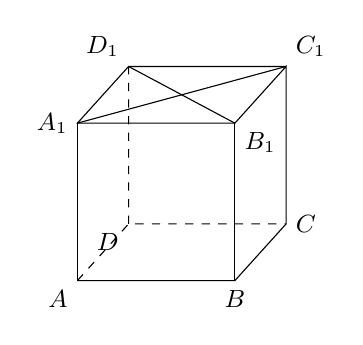
\begin{tikzpicture}[x=1cm, y=1cm, font=\small]
  \coordinate (A)  at (0,0);
  \coordinate (B)  at (2,0);
  \coordinate (C)  at (2.65,0.72);
  \coordinate (D)  at (0.65,0.72);
  \coordinate (A1) at (0,2);
  \coordinate (B1) at (2,2);
  \coordinate (C1) at (2.65,2.72);
  \coordinate (D1) at (0.65,2.72);

  % 可见棱
  \draw (A) -- (B) -- (C) -- (C1) -- (B1) -- (A1) -- (D1) -- (C1);
  \draw (A) -- (A1);
  \draw (B) -- (B1);
  % 源图中的隐藏棱
  \draw[dashed] (A) -- (D) -- (C) (D) -- (D1);
  % 顶面两条对角线
  \draw (A1) -- (C1);
  \draw (D1) -- (B1);

  \node[below left] at (A) {$A$};
  \node[below] at (B) {$B$};
  \node[right] at (C) {$C$};
  \node[below left] at (D) {$D$};
  \node[left] at (A1) {$A_1$};
  \node[below right] at (B1) {$B_1$};
  \node[above right] at (C1) {$C_1$};
  \node[above left] at (D1) {$D_1$};
\end{tikzpicture}
\end{center}
\nopagebreak[4]
\Needspace{4\baselineskip}
\textbf{解析}

\gksubpart{(1)}

取标准坐标 $A=(0,0,0),B=(1,0,0),C=(1,1,0),D=(0,1,0)$，顶部顶点的 $z$ 坐标为 $1$，$P=(1,1,m)$。平面 $BDD_1B_1$ 的方程为 $x+y=1$，其法向量为 $(1,1,0)$。直线 $AP$ 的线面角正切为 $\sqrt2/m$，令其为 $3\sqrt2$，得 $m=1/3$。

\gksubpart{(2)}

设 $Q=(t,t,1)\in A_1C_1$，则 $\overrightarrow{D_1Q}=(t,t-1,0)$、$\overrightarrow{AP}=(1,1,m)$。将 $D_1Q$ 投影到含 $AP$ 的平面后，其与 $AP$ 的点积仍为原向量点积 $2t-1$。取固定 $t=1/2$ 即得垂直关系，对任意 $m$ 都成立。

\gkanswer{答案（1）：$m=1/3$。}

\gkanswer{答案（2）：存在；}

\end{answer}
\begin{answer}
\gksolhead{19}{}

\textbf{题目}：

在某校举行的数学竞赛中，全体参赛学生的竞赛成绩近似服从正态分布 $N(70,100)$。已知成绩在 $90$ 分以上（含 $90$ 分）的学生有 $12$ 名。

（1） 试问此次参赛学生总数约为多少人？

（2） 若该校计划奖励竞赛成绩排在前 $50$ 名的学生，试问设奖的分数线约为多少分？

可供查阅的（部分）标准正态分布表 $\Phi(x_0)=P(x<x_0)$：

\begin{center}
\begin{tabular}{lrrrrr}
\toprule
$x_0$ & 0 & 1 & 2 & 3 & 4 \\
\midrule
1.2 & 0.8849 & 0.8869 & 0.888 & 0.8907 & 0.8925 \\
1.3 & 0.9032 & 0.9049 & 0.9066 & 0.9082 & 0.9099 \\
1.4 & 0.9192 & 0.9207 & 0.9222 & 0.9236 & 0.9251 \\
1.9 & 0.9713 & 0.9719 & 0.9726 & 0.9732 & 0.9738 \\
2.0 & 0.9772 & 0.9778 & 0.9783 & 0.9788 & 0.9793 \\
2.1 & 0.9821 & 0.9826 & 0.9830 & 0.9834 & 0.9838 \\
\bottomrule
\end{tabular}
\end{center}

\begin{center}
\begin{tabular}{lrrrrr}
\toprule
$x_0$ & 5 & 6 & 7 & 8 & 9 \\
\midrule
1.2 & 0.8944 & 0.8962 & 0.8980 & 0.8997 & 0.9015 \\
1.3 & 0.9115 & 0.9131 & 0.9147 & 0.9162 & 0.9177 \\
1.4 & 0.9265 & 0.9278 & 0.9292 & 0.9306 & 0.9319 \\
1.9 & 0.9744 & 0.9750 & 0.9756 & 0.9762 & 0.9767 \\
2.0 & 0.9798 & 0.9803 & 0.9808 & 0.9812 & 0.9817 \\
2.1 & 0.9842 & 0.9846 & 0.9850 & 0.9854 & 0.9857 \\
\bottomrule
\end{tabular}
\end{center}

\Needspace{4\baselineskip}
\textbf{解析}

\gksubpart{(1)}

分数标准差为 $10$，$90$ 分对应 $z=2$。表给右尾概率 $1-0.9772=0.0228$，总人数约为 $12/0.0228\approx526$。

\gksubpart{(2)}

前 $50$ 名对应累计概率约 $1-50/526.3\approx0.905$，由表取 $z\approx1.31$，分数线约 $70+10(1.31)=83.1$。

\gkanswer{答案（1）：约 $526$ 人。}

\gkanswer{答案（2）：约 $83.1$ 分。}

\end{answer}
\begin{answer}
\gksolhead{20}{}

\textbf{题目}：

设 $A,B$ 分别为椭圆 $\dfrac{x^2}{a^2}+\dfrac{y^2}{b^2}=1\ (a,b>0)$ 的左、右顶点，椭圆长半轴的长等于焦距，且 $x=4$ 为它的右准线。

（1） 求椭圆的方程；

（2） 设 $P$ 为右准线上不同于点 $(4,0)$ 的任意一点，若直线 $AP,BP$ 分别与椭圆相交于异于 $A,B$ 的点 $M,N$，证明点 $B$ 在以 $MN$ 为直径的圆内。

\Needspace{4\baselineskip}
\textbf{解析}

\gksubpart{(1)}

长半轴长等于焦距，故 $a=2c$；右准线 $a^2/c=4$ 给 $a=2,c=1$，于是 $b^2=3$，椭圆为 $x^2/4+y^2/3=1$。

\gksubpart{(2)}

\Needspace{5\baselineskip}
令右准线上 $P=(4,t)$，$t\ne0$。记 $B=(2,0)$。直线 $AP$ 上除 $A$ 外的椭圆交点 $M$、直线 $BP$ 上除 $B$ 外的交点 $N$ 满足
\nopagebreak[4]
\[
\overrightarrow{BM}=\left(-\frac{4t^2}{t^2+27},\frac{18t}{t^2+27}\right),\qquad
\overrightarrow{BN}=\left(-\frac{12}{t^2+3},-\frac{6t}{t^2+3}\right).
\]

\Needspace{5\baselineskip}
因此
\nopagebreak[4]
\[
\overrightarrow{BM}\cdot\overrightarrow{BN}
=-\frac{60t^2}{(t^2+27)(t^2+3)}<0.
\]

故 $\angle MBN$ 为钝角。由泰勒斯定理的逆定理，$B$ 严格位于以 $MN$ 为直径的圆内，题设结论成立。

\gkanswer{答案（1）：$\frac{x^2}{4}+\frac{y^2}{3}=1$。}

\gkanswer{答案（2）：见解析版}

\end{answer}
\begin{answer}
\gksolhead{21}{}

\textbf{题目}：

设 $x=3$ 是函数 $f(x)=(x^2+ax+b)e^{3-x}\ (x\in\mathbb R)$ 的一个极值点。

（1） 求 $a$ 与 $b$ 的关系式（用 $a$ 表示 $b$），并求 $f(x)$ 的单调区间；

（2） 设 $a>0$，$g(x)=\left(a^2+\dfrac{25}{4}\right)e^x$。若存在 $\xi_1,\xi_2\in[0,4]$ 使得 $|f(\xi_1)-g(\xi_2)|<1$ 成立，求 $a$ 的取值范围。

\Needspace{4\baselineskip}
\textbf{解析}

\gksubpart{(1)}

\Needspace{5\baselineskip}
对 $f(x)=(x^2+ax+b)e^{3-x}$ 求导，令 $f'(3)=0$ 得 $b=-2a-3$。此时
\nopagebreak[4]
\[
f'(x)=-e^{3-x}(x-3)(x+a+1).
\]

还需排除 $a=-4$，因为此时 $x=3$ 为二重驻点而不是极值点。若 $a>-4$，单调区间依次为 $(-\infty,-a-1)$ 递减、$(-a-1,3)$ 递增、$(3,+\infty)$ 递减；若 $a<-4$，则 $(-\infty,3)$ 递减、$(3,-a-1)$ 递增、$(-a-1,+\infty)$ 递减。

\gksubpart{(2)}

在 $a>0$ 时，$-a-1<0$，故 $f$ 在 $[0,3]$ 递增、$[3,4]$ 递减，最大值为 $f(3)=a+6$。$g(x)=(a^2+25/4)e^x$ 在 $[0,4]$ 的最小值为 $a^2+25/4$。两值间距为 $a^2-a+1/4=(a-1/2)^2$；存在一对函数值距离小于 $1$ 当且仅当该间距小于 $1$，即 $0<a<3/2$。

\gkanswer{答案（1）：$b=-2a-3$；}

\gkanswer{答案（2）：$0<a<3/2$。}

\end{answer}